\documentclass[../mainfile.tex]{subfiles}



\begin{document}
\section{Construction of a Brownian motion}
\subsection{Goal}
We want to construct a one-dimensional Brownian Motion, that is, we want to find a probability space and a collection of random variables $(B_t)_{t \geq 0}$ ($t$ is indexed over $\mathbb{R}_+$) such that:
\begin{enumerate}
\item $B_0=0$ almost surely.
\item $B$ has independent and stationary increments.
\begin{enumerate}
\item Stationary increments: For all $t,h \geq 0$, we have $B(t+h)-B(t) \sim B(h)$.
\item Independent increments: For all positive integers $k$ and times $0 \leq t_1 < t_2 < \dots < t_k$ in $\mathbb{R}_+$, the $k$ increments $B(t_1)-B(0), B(t_2)-B(t_1), \dots , B(t_k)-B(t_{k-1})$ are independent random variables. 
\end{enumerate}
\item $B_t \sim \mathcal{N}(0,t)$ for all $t \in \mathbb{R}_+$.
\item There exists a set of probability $1$, such that on this set $t \mapsto B_t$ is a continuous function. \textit{(Hardest part in the proof)}
\end{enumerate}
\subsection{Preliminaries}
Surprisingly, we only require a bare minimum of prerequisites in order to perform the construction of a Brownian motion. Namely:
\begin{enumerate}
\item There exists a probability space on which we can define a countable family of independent centered normal variables, i.e. a collection $N_j \sim \mathcal{N}(0,1)$ for all $j \in \mathbb{N}$. 
\item If $N \sim \mathcal{N}(0,1)$, then $aN \sim \mathcal{N}(0,a^2)$ for all constants $a$. 
\item $X \sim \mathcal{N}(0, \sigma_X^2), \ Y \sim \mathcal{N}(0, \sigma_Y^2)$ and if $X$ and $Y$ are independent, then $X+Y \sim \mathcal{N}(0, \sigma_X^2 + \sigma_Y^2)$. 
\item If $N \sim \mathcal{N}(0, \sigma^2)$ and $N' \sim \mathcal{N}(0, \sigma^2)$ and $N,N'$ are independent, then the two random variables 
\begin{align*}
\frac{N+N'}{2} \text{ and } \frac{N-N'}{2}
\end{align*}
are independent with common law $\mathcal{N}(0, \sigma^2/2)$, notice that their sum adds up to $N$. This can be seen as a \textit{decomposition law}. 
\end{enumerate}
\newpage
\subsection{Construction}
\subsubsection{Notation and warm-up}
For every $n \in \mathbb{N}$ we set $\mathcal{I}_n:= \{ [j2^{-n}, (j+1)2^{-n}] : j \in \mathbb{N}\}$ and we define $\mathcal{I}:= \cup_{n \in \mathbb{N}} \mathcal{I}_n$ (everything nice and countable so far). An element of $\mathcal{I}$ is therefore an interval $I_{j,n}=[j2^{-n},(j+1)2^{-n}]$ for some $n,j$. For $I \in \mathcal{I}$ we set $r(I)$ and $l(I)$ to be closed right half, respectively the closed left half of $I$. 
\\\\
For clarity purposes, here are two examples: Let $I_{j,n}=[j2^{-n},(j+1)2^{-n}]$ as above, then
\begin{align*}
l(I_{j,n})&=I_{2j,n+1} =[j2^{-n}, (2j+1)2^{-n-1}] \\
r(I_{j,n})&=I_{2j+1,n+1}=[(2j+1)2^{-n-1},(j+1)2^{-n}]
\end{align*}
For the rest of the construction we consider a probability space $(\Omega, \mathcal{F}, \mathbb{P})$ that contains a countable collection of independent centered Gaussian random variables, with 
\begin{equation*}
\begin{rcases}
N_j &\sim \mathcal{N}(0,1) \text{ for all } j \in \mathbb{N}.\\
N_{j,n} &\sim \mathcal{N}(0, 2^{-n}) \text{ for all } j,n \in \mathbb{N}. 
\end{rcases}
\text{Independent}
\end{equation*}
\subsubsection{Construction on integer times}
We first construct the values of the Brownian Motion at \textbf{integer times}. This is easy, we simply define the values of the process $A$ (that we want to be a Brownian motion) as follows: $A(0)=0$, $A(1)=N_1$ ,$A(2)=A(1)+N_2=N_1+N_2$ and $A(j)=A(j-1)+N_j=N_1 + \dots + N_j$. In particular we have $A(j)\sim \mathcal{N}(0,j)$, for every increment $A(j)-A(j-1)=N_j \sim \mathcal{N}(0,1) \sim A(1)$ and naturally all increments are independent because the $N_j$'s are, as desired. 
\begin{figure}[hbtp]
\centering
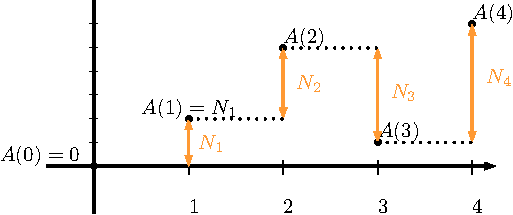
\includegraphics[scale=1]{figure1.pdf}
\caption{Construction on integer values with increments $N_i$ displayed.}
\end{figure}
\newpage
\subsubsection{Construction on half integers times}
Next we construct the values of the Brownian motion at \textbf{half integers times}. We introduce the notation $\Delta_I$, which will denote what will be the increment of the Brownian Motion on the interval $I$. 
\\\\
We look at each interval $I_{j,0}=[j,j+1]$ separately, we already know the values of the Brownian Motion on such intervals, we introduce the more convenient notation $\Delta_{j,0}:=\Delta_{I_{j,0}}$ and we already know that 
\begin{align*}
\Delta_{j,0}=A(j+1)-A(j)=N_j \sim \mathcal{N}(0,1).
\end{align*}
For $N_{j,0} \sim \mathcal{N}(0,2^{-0}) = \mathcal{N}(0,1)$ we know that 
\begin{align*}
\frac{\Delta_{j,0}+N_{j,0}}{2} \text{ and } \frac{\Delta_{j,0}-N_{j,0}}{2}
\end{align*}
are two independent RV with common law $\mathcal{N}(0,2^{-1})$ whose sum is $\Delta_{j,0}$. 
\\\\
We now define: 
\begin{align*}
A\left(j + \frac{1}{2}\right) := A(j) + \left( \frac{\Delta_{j,0}+N_{j,0}}{2} \right) \sim \mathcal{N}\left(0,j+ \frac{1}{2}\right). \tag{*}
\end{align*}
This definition guarantees now that for the left respectively right half of $[j,j+1]$ we get:
\begin{align*}
\Delta_{[j,j+1/2]} &= A(j+1/2)-A(j)= \frac{\Delta_{j,0}+N_{j,0}}{2} \sim \mathcal{N}(0,2^{-1}), \\
\Delta_{[j+1/2,j+1]} &= A(j+1)-A(j+1/2) \\
& = A(j+1)-A(j)-\frac{\Delta_{j,0}+N_{j,0}}{2} \\
& = \Delta_{j,0}-\frac{\Delta_{j,0}+N_{j,0}}{2}  = \frac{\Delta_{j,0}-N_{j,0}}{2} \sim \mathcal{N}(0,2^{-1}).
\end{align*}
So we have again $A(j+1/2) \sim \mathcal{N}(0, j+1/2)$, all increments satisfy moreover that $A(j+1/2)-A(j) \sim \mathcal{N}(0,1/2) \sim A(1/2)$ are therefore stationary and by the above calculations of the decomposition we also have that the increments are independent. 
\\\\
\textbf{Remark:} Notice that the equation (*) above can be rewritten as 
\begin{align*}
A \left( j + \frac{1}{2} \right) = \frac{A(j)+A(j+1)}{2} + \frac{N_{j,0}}{2}
\end{align*}
this equation gives rise to a more geometric interpretation of our construction, see figure 2. 
\newpage
\begin{figure}[hbtp]
\centering
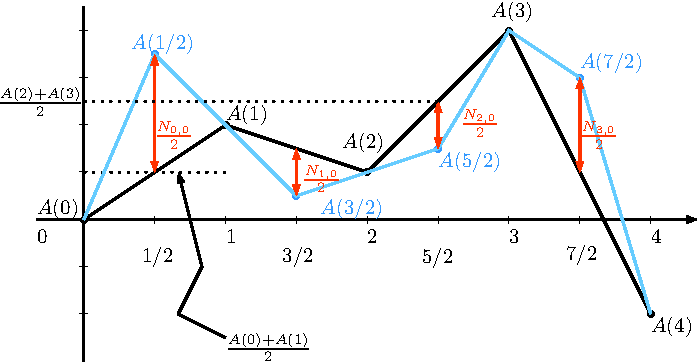
\includegraphics[scale=1]{figure2.pdf}
\caption{Geometric interpretation of our construction on the half integers}
\end{figure}
Notice that the blue and the black lines are merely for illustrative purposes. Moreover it's important to remark that $\frac{1}{2}N_{i,0} \sim \mathcal{N}(0,1/4)$ for all $i \in \mathbb{N}$ and also $((A(i)+A(i+1))/2 \sim \mathcal{N}(0, i+ 1/4)$. 
\subsection{Inductive construction on dyadics}
We iterate over $n \in \mathbb{N}$. Let us assume that we know (for a fixed $n \in \mathbb{N}$) the values of $A(j2^{-n})$ for all $j \in \mathbb{N}$. In particular,  we know the increments $\Delta_{j,n}$ for all $j \in \mathbb{N}$ and all $(\Delta_{j,n})_{j \geq 0}$ are i.i.d. with common law $\mathcal{N}(0, 2^{-n})$. 
\\\\
We then take again $(N_{j,n})_{j \geq 0 }$ i.i.d. $\mathcal{N}(0, 2^{-n})$ and independent of $(\Delta_{j,n})_{j \geq 0 }$. We then define for all intervals $I=I_{j,n}=[j2^{-n},(j+1)2^{-n}]$ the increments $\Delta_{2j,n+1}$, $\Delta_{2j+1,n+1}$ on $l(I)$ respectively on $r(I)$ by:
\begin{align*}
\Delta_{2j,n+1}:= \frac{\Delta_{j,n}+N_{j,n}}{2}, \ \Delta_{2j+1,n+1} := \frac{\Delta_{j,n}-N_{j,n}}{2}.
\end{align*}
The previous arguments (same as on half integers) shows that this time $(\Delta_{j,n+1})_{j \geq 0}$ are i.i.d. $\mathcal{N}(0,2^{-(n+1)})$. Also, just as in the previous step we define
\begin{align*}
A( \text{middle}(I_{j,n})) := A(j2^{-n})+ \Delta_{2j,n+1} \sim \mathcal{N}(0, (j+1/2)2^{-n}). 
\end{align*}
With this construction we have now a collection of random variables $(A(q))_{q \in \mathcal{D}}$ where $\mathcal{D}=\{j2^{-n},j \geq 0, n \geq 0\}$ denotes the set of the dyadics. We have the properties $A(0)=0$ almost surely, $A(q) \sim \mathcal{N}(0,q)$ on $\mathcal{D}$ and it has stationary independent increments on $\mathcal{D}$. 
\newpage
\subsection{Continuous extension to $\mathbb{R}_+$
}
We will see that almost surely the function $\mathcal{D} \ni q \mapsto A(q)$ can be extended into a continuous function $t \mapsto \tilde{A}(t)$ on $\mathbb{R}_+$ and we will show that indeed $t \mapsto \tilde{A}(t)$ is a Brownian motion. \\
\\
We define for all $n \in \mathbb{N}$, the function $f_n(t)$ where $t \geq 0$ to be the linear interpolation of $A(0), A(1\cdot 2^{-n}), A(2\cdot 2^{-n}), \dots ,  A(j2^{-n}) , \dots$ (i.e. linear on each $I_{j,n})$. 
\\\\
Our goal is to show that $f_n$ converges uniformly to some continuous function $f$ on any compact interval $[0,K]$, where $K$ is an integer. 
\\
In order to achieve this goal, we notice that the function $f_{n+1}-f_n$ is
\begin{itemize}
\item a continuous linear function on each interval $I_{j,n+1}$.
\item equal to $0$ at each $j/2^n$ for all $j$. 
\item equal to $N_{j,n}/2$ at each middle point of $I_{j,n}$. 
\end{itemize}
\begin{figure}[hbtp]
\centering
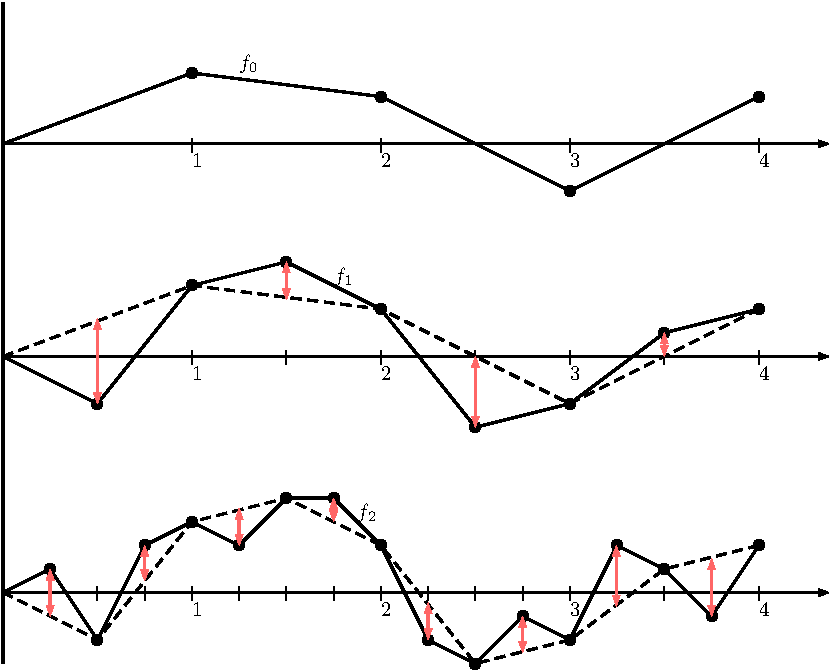
\includegraphics[scale=.742]{figurewend.pdf}
\caption{Illustration of the iterative construction: First on the integers, then on the half-integers and so on. The increment of $f_n$ on the interval $I_{j,n}=[j2^{-n},(j+1)2^{-n}]$ is $\Delta_{j,n}$. The difference $f_{n+1}-f_n$ at the middle point of each $I_{j,n}$ is $N_{j,n}/2$ (red), and at each end point of $I_{j,n}$ is zero.}
\end{figure}
\newpage
With figure 3 in mind we obtain for all integers $K$ and $x \geq 1$,
\begin{align*}
\mathbb{P}( \max_{[0,K]} |f_{n+1}-f_n|  \geq x2^{-n/2} ) \overset{1)}= \mathbb{P}( \exists j \leq K2^n-1 : |N_{j,n}|  \geq 2x2^{-n/2} ) 
\\
\overset{2)}\leq \sum_{j \leq K2^n-1} \mathbb{P}(|N_{j,n}| \geq 2x2^{-n/2}) \overset{3)}= K2^n \mathbb{P}(|N_1| \geq 2x) \overset{4)}\leq K2^n e^{-2x^2}.
\end{align*}
Where we used:
\begin{enumerate}
\item If the maximum is attained, then it's attained at the mid point of the intervals (see figure 3) where its value is $N_{j,n}/2$ (it cannot be at the start/end points because there $f_{n+1}-f_n \equiv 0)$. Moreover we translate the interval $[0,K]$ for $I_{j,n}=[j2^{-n},(j+1)2^{-n}]$ i.e. $j$ must run from $0$ to $K2^n-1$. 
\item Union bound.
\item  We have $N_{j,n}$ i.i.d. $\mathcal{N}(0,2^{-n})$ which implies that $2^{n/2} N_{j,n} \sim \mathcal{N}(0,1)$ and still i.i.d. so we just take $N_1 \sim \mathcal{N}(0,1)$ (independent of $j$). 
\item Very crude upper bound for a standard Gaussian, easy to show. 
\end{enumerate}
If we now choose $x=n\in \mathbb{N}_{ \geq 1}$ in our estimate above, we  notice that the upper bound is summable, i.e. $\sum_{n \geq 1}\mathbb{P}( \max_{[0,K]} |f_{n+1}-f_n|  \geq n2^{-n/2} ) < \infty$. By the Borel-Cantelli Lemma, we can conclude that almust surely,  there exists a (random) $n_0=n_0(\omega)$ such that for all $n \geq n_0$ we have 
\begin{align*}
|f_{n+1}-f_n| \leq n2^{-n/2} \text{ on } [0,K].
\end{align*}
Since $\sum n2^{-n/2}< \infty$, it is very easy to conclude from the above that $(f_n)_{n \geq 1}$ is uniformly Cauchy on $[0,K]$ (since the sum over all increments $|f_{n+1}-f_n|$ converges, we must have for large enough $p,n$ that $|f_p-f_n|$ converges to $0$). \\
\\
Since $(f_n)_{n \geq 1}$ is uniformly Cauchy on $[0,K]$ we know that it must converge uniformly on the interval  $[0,K]$ as $n \to \infty$ to some function $f$, and that this limit $f$ is almost surely a continuous function on $[0,K]$. \\
\\
We remark that this is true for each integer $K$, so we can interchange "almost surely" and "for all $K$" (recall that $\forall k, \mathbb{P}(A_k)$ is 'weaker' than $\mathbb{P}(\forall k, A_k)= \mathbb{P}(\cap_k A_k)$) to conclude that: \textit{Almost surely, the function $f_n$ converges uniformly on any compact subset of $\mathbb{R}_+$ to a limiting function $f$, and this limiting function $f$ is continuous on $\mathbb{R}_+$.} We used that $\forall k \geq 0$ (integer i.e. countable) $\mathbb{P}(A_k^c)=0$ then $\mathbb{P}(\cup_{k \in \mathbb{N}} A_k^c) \leq \sum_{k \in \mathbb{N}} \mathbb{P}(A_k^c)=0$ i.e. $\mathbb{P}(\cap_{k \in \mathbb{N}} A_k)=1$. 
\newpage
\subsubsection{The continuous extension is a Brownian motion}
We will now prove that the law of the stochastic process $(f(t))_{t \geq 0}$ that has been constructed in the previous section is indeed that of a Brownian motion. We do already know that it is continuous and that $f(0)=0$ almost surely. It remains to check that for any $0=t_0<t_1< \dots < t_k$, the random variables 
\begin{align*}
f(t_1)-f(t_0),f(t_2)-f(t_1), \dots , f(t_k)-f(t_{k-1})
\end{align*}
are independent, and that the law of $f(t+h)-f(t)$ is a centered Gaussian variable with variance $h$. \\
\\
To establish this, we first choose for each time $t_l$ where $l=1, \dots,k$, a sequence $t_l(n)$ of dyadic times that converges to $t_l$. (For instance, we take $t_l(n)$ to be the smallest multiple of $2^{-n}$ that is larger than $t_l$). Because of the continuity of $f$, we know that almost surely, $f(t_l(n)) \to f(t_l)$ as $n \to \infty$. This readily implies that the random variables 
\begin{align*}
f(t_1)-f(t_0),f(t_2)-f(t_1), \dots , f(t_k)-f(t_{k-1})
\end{align*}
are independent as the almost sure limits of the independent random variables
\begin{align*}
f(t_1(n)),f(t_2(n))-f(t_1(n)), \dots , f(t_k(n))-f(t_{k-1}(n)).
\end{align*}
Moreover we know that $f(t_l(n))-f(t_{l-1}(n))$ is a centered Gaussian with variance $t_l(n)-t_{l-1}(n)$. Furthermore, $t_l(n)-t_{l-1}(n)$ converges to $t_l-t_{l-1}$ as $n \to \infty$. Therefore we get for all $\lambda \in \mathbb{R}$,  that
\begin{align*}
\mathbb{E}( \exp(i \lambda (f(t_l)-f(t_{l-1}))) = \lim_{n \to \infty} \mathbb{E}( \exp(i \lambda (f(t_l(n))-f(t_{l-1}(n)))) \\
= \lim_{n \to \infty} \exp( - \lambda^2/(2(t_l(n)-t_{l-1}(n)))) = \exp( - \lambda^2/(2(t_l-t_{l-1}))).
\end{align*}
This establishes that $f(t_l)-f(t_{l-1})$ is indeed a centered Gaussian random variable with variance $t_l-t_{l-1}$. This concludes the construction and shows that the process $f$ is indeed a Brownian motion. 
\begin{rem} We see that this last part of the proof is in essence nothing more than using that the set of dyadic times $\mathcal{D}$ is dense in $\mathbb{R}_+$, i.e. we can approximate times $t \in \mathbb{R}_+$ by times $\tilde{t}$ in $\mathcal{D}$.
\end{rem}
\newpage
\subsection{Kolmogorov's continuity criterion}
Since it matches the current presentation quite well, we will also briefly discuss Kolmogorov's continuity criterion. The underlying question one should have in mind is \textit{if continuity can be read off from the law of a stochastic process or not}. Certainly the answer is no, because it is quite easy to construct two stochastic processes which have the same law, one being continuous (always equal to $0$) and the other having jumps.\\
\\
However, we do add quite a bit more subtlety to this question if we consider \textit{continuous modifications} of a stochastic process. Assume we are given the law of a stochastic process $(X_t)_{t \in I}$. We can then check whether it is possible to find some probability space, and some random process $(Y_t)_{t \in I}$ with this given law, such that there exists a measurable set with probability $1$, such that for all $\omega$ in this set, $t \mapsto Y_t$ is continuous on $I$. It is possible to show that for all $t \in I$ we have $X_t=Y_t$ almost surely (i.e. $\forall t \in I, \ \mathbb{P}(X_t=Y_t)=1$), we then say that the process $Y$ is a continuous modification of $X$. 
\begin{thm}[Kolmogorov's continuity criterion] If $(X_t)_{t \geq 0}$ is a stochastic process such that for all $T >0$, there exists $\epsilon >0, \alpha >0, C>0$ such that for all $t,s \in [0,T]$ we have 
\begin{align*}
\mathbb{E}(|X_t-X_s|^\alpha) \leq C|t-s|^{1 + \epsilon}, \tag{$\varsigma$}
\end{align*}
then $X$ admits a continuous modification. 
\end{thm}
\begin{rem} Before we write down the proof, it is important to mention that we follow very similar arguments as in the construction of a Brownian motion to establish the proof. 
\end{rem}
\begin{proof}
Let us assume that $Z_q=X_q$ for all dyadics $q \in \mathcal{D}$. Let us try to bound $|Z_{(j+1)2^{-n}}-Z_{j2^{-n}}|$ for all $j \leq 2^nT-1$. 
\begin{align*}
\mathbb{P}( \exists j \leq T2^n-1: |Z_{(j+1)2^{-n}}-Z_{j2^{-n}}| \geq x_n) \leq \sum_{j \leq T2^n-1} \mathbb{P}(|X_{(j+1)2^{-n}}-X_{j2^{-n}}|^\alpha \geq x_n^\alpha ) \\
\overset{\text{Markov}}\leq \sum_{j \leq T2^n-1} \frac{1}{x_n^\alpha} \mathbb{E}(|X_{(j+1)2^{-n}}-X_{j2^{-n}}|^\alpha) \overset{\varsigma}\leq T2^n C \frac{(2^{-n})^{1 + \epsilon}}{x_n^\alpha} = TC \frac{2^{-n \epsilon}}{x_n^\alpha} = TC 2^{-n \epsilon /2}
\end{align*}
Where in the last step we specialized on $x_n= 2^{-n \epsilon / (2 \alpha)}$. Since $\sum 2^{-n \epsilon/2} < \infty$, we have by the Borel-Cantelli Lemma that almost surely, there exists $n_0(\omega)$ such that for all $n \geq n_0(\omega), j \leq T2^n-1$ we have 
\begin{align*}
|X_{(j+1)2^{-n}}-X_{j2^{-n}}| < 2^{-n \epsilon /(2 \alpha)}
\end{align*}
\newpage
We now define $f_n$ to be the linear interpolation of the values of $X$ on the dyadics $\mathcal{D}$ (multiples of $2^{-n}$). \\\\
$\max ( |f_{n+1}-f_n|)$ on $[0,T]$ is attained at one of the middle points of $I_{j,n}$ and is therefore bounded by the maximum over all $j \leq 2^{(n+1)}T-1$, thus almost surely there exists $n_0(\omega)$, for all $n \geq n_0$ such that \begin{align*}
\max_{[0,T]} |f_{n+1}-f_n| \leq 2^{-\frac{(n+1) \epsilon}{2 \alpha}}.
\end{align*}
Since $\sum 2^{-n \epsilon/( 2 \alpha)} < \infty$, we get that the series $\sum |f_{n+1}-f_n|$ is uniformly summable and thus $(f_n)_{n \in \mathbb{N}}$ is uniformly Cauchy on $[0,T]$. Therefore there exists a continuous function $f$ on $[0,T]$ such that $f_n \to f$ uniformly on $[0,T]$.
\\\\
We now claim that for all fixed $t>0$ we have $f(t)=X(t)$ almost surely, that is $f$ is a continuous modification of $X$. To this extent let $q_n(t)$ be a sequence of dyadics that converges to $t$. Since $f$ is almost surely continuous at $t$ we have (almost surely)
\begin{align*}
f(t)=\lim_{n \to \infty} f(q_n(t)) = \lim_{n \to \infty} X(q_n(t)). \tag{*}
\end{align*}
On the other hand, by $( \varsigma)$ we also have for all $\delta >0$
\begin{align*}
\mathbb{P}(|X(t)-X(q_n(t))| > \delta ) &\leq \delta^{-\alpha} \mathbb{E}(|X(t)-X(q_n(t))|^\alpha) \\ &\leq C \delta^{- \alpha} |t-q_n(t)|^{1 + \epsilon} \overset{n \to \infty}\longrightarrow 0,
\end{align*}
so we have $X(q_n(t)) \to X(t)$ in Probability as $n \to \infty$. Since the almost sure convergence in (*) above implies convergence is Probability and the limit of convergence in probability is unique we must have that $f(t)=X(t)$ almost surely. 
\end{proof}
\begin{lem} Kolmogorov's continuity criterion is satisfied by the law of Brownian motion. 
\end{lem}
\begin{proof}
We know that $B_t-B_s \sim \mathcal{N}(0,t-s)$ for all $t>0, s<t$. We first notice that $\mathbb{E}((B_t-B_s)^2)=|t-s|^1$, so we have no chance for this exponent to satisfy Kolmogorov's continuity criterion. However, we can easily see that $\sqrt{t-s} B_1 \sim \mathcal{N}(0,t-s)$ and consequently
\begin{align*}
\mathbb{E}((B_t-B_s)^4)=\mathbb{E}( (\sqrt{t-s} B_1)^4)= |t-s|^2 \underbrace{\mathbb{E}(B_1^4)}_{< \infty}
\end{align*}
So we choose $\epsilon=1, \alpha=4, C= \mathbb{E}(B_1)^4$ and conclude by Kolmogorv's continuity criterion.
\end{proof}
\newpage
\begin{rem}
It is possible to adapt the proof of Kolmogorov's continuity criterion to show that if the conditions are satisfied, then the modification will not only be continuous, but also $\gamma$-Hölder continuous for any $\gamma < \epsilon/\alpha$ in the sense that for all $T>0$, there almost surely exists $C=C(T,\gamma)$ such that for all $0 \leq s < t \leq T$ we have
\begin{align*}
|B_t-B_s| \leq C|t-s|^\gamma. 
\end{align*}
Since for Brownian motion (using the same argument as in the proof of the lemma before), one can take $\alpha = 2k$ and $\epsilon = k-1$ this shows that Brownian motion is almost surely Hölder continuous of exponent $\gamma$ for all $\gamma < 1/2$. We will later establish that Brownian motion is not Hölder of exponent $1/2$. 
\end{rem}
\newpage
\subsection{Brownian motion as a Gaussian process, and consequences}
Before we give another approach to constructing a Brownian motion, which will be more from a Functional Analytic point of view,  it will be fruitful to introduce Gaussian processes in order to describe Brownian motion. 
\begin{defn} A random vector $(X_1,  \dots , X_n) \in \mathbb{R}^n$ is a centered Gaussian vector if any linear combination of the $X_i$'s is a centered Gaussian random variable. 
\end{defn} 
We can make some useful remarks (that should be reminders):
\begin{itemize}
\item If $N_1, \dots , N_k$ are i.i.d. centered Gaussian random variables, then any vector whose entries are (fixed) linear combinations of the $N_1, \dots , N_k$ is a centered Gaussian vector. In other words, if there exists $Q$ a $n \times n$ Matrix such that $(X_1, \dots , X_n)= (N_1, \dots , N_d) \cdot Q$, then $(X_1, \dots , X_n)$ is a Gaussian vector. 
\item A nice useful property is that the law of a centered Gaussian vector $X$ is completely characterized by its covariance matrix $\sum_X=( \mathbb{E}(X_iX_j))_{1 \leq i,j \leq n}$. 
\item If $(X_1, \dots , X_n)$ is a centered Gaussian vector and if for some $n_0 < n$, one has $\mathbb{E}(X_i,X_j)=0$ for all $1 \leq i \leq n_o < j \leq n$, then the vectors $(X_1, \dots , X_{n_0})$ and $(X_{n_0+1}, \dots , X_n)$ are independent.
\end{itemize}
\begin{defn} A stochastic process $(X_t)_{t \in I}$ is said to be a centered Gaussian process for all $n \in \mathbb{N}$ and for all $t_1, \dots , t_k \in I$ the finite dimensional vector $(X_{t_1}, \dots , X_{t_n})$ is a Gaussian vector. The covariance function of a stochastic process $X=(X_t)_{t \in I}$ is the function $\sum_X$ defined on $I \times I$ by $\sum_X(s,t)= \mathbb{E}(X_sX_t)$. 
\end{defn}
\begin{rem} We know that the finite-dimensional distributions of $X$ are completely characterized by $\sum_X$, so that the law of the whole process is also characterized by the covariance function $\sum_X$. \textit{(Recall that the law of a stochastic process is determined by its finite-dimensional distributions).}
\end{rem}
The important statement in this subsection is the following:
\begin{prop} A Brownian Motion $(B_t)_{t \geq 0}$ is a (centered) Gaussian process with covariance function given by 
\begin{align*}
\Sigma_B(s,t)= \mathbb{E}(B_tB_s)= \min(s,t).
\end{align*}
\end{prop}
\newpage
\begin{proof}
Let us choose $t_1 < t_2< \dots < t_k$ for $k \in \mathbb{N}$ and $\lambda_1, \dots , \lambda_k \in \mathbb{R}$. We want to show that $\lambda_1 B_{t_1}+ \dots + \lambda_k B_{t_k}$ is a centered Gaussian variable. This is easy because we can write this as a linear combination of the independent centered Gaussian variables 
\begin{align*}
B_{t_1}, (B_{t_2}-B_{t_1}), \dots , (B_{t_k}-B_{t_k-1})
\end{align*}
using telescopic sums for example. Let us now assume that $s<t$, then 
\begin{align*}
\mathbb{E}(B_tB_s)&= \mathbb{E}((B_s+B_t-B_s)B_s) = \mathbb{E}(B_s^2) + \mathbb{E}((B_t-B_s)B_s) \\ 
&= s + \mathbb{E}((B_t-B_s)(B_s-B_0))= s + \mathbb{E}(B_t-B_s)\mathbb{E}(B_s)= s
\end{align*}
where we used that for $s<t$, $B_t-B_s$ is independent of $B_s-B_0=B_s$.
\end{proof}
\begin{cor}[Characterization] $(B_t)_{t \geq 0}$ is a Brownian motion if and only if $t \mapsto B_t$ is continuous on an event of probability $1$ \textbf{and} $(B_t)_{t \geq 0}$ is a Gaussian process with covariance function $\mathbb{E}(B_tB_s)= \min(s,t)$. 
\end{cor}
\subsubsection{Some invariance properties of Brownian motion} The following facts are immediate consequences of the previous description of a Brownian motion as a centered Gaussian process with covariance function $\mathbb{E}(B_sB_t)=s \wedge t$. 
\begin{prop} Let $(B_t)_{t \geq 0}$ be a one-dimensional Brownian motion, then:
\begin{itemize}
\item (Scaling invariance). For every $a>0$, the process $(a^{-1} B_{a^2t})_{t \geq 0}$ is a Brownian motion.
\item (Inversion invariance). The process $(tB_{1/t})_{t > 0}$ is distributed like $(B_t)_{t >0}$.
\item (Invariance under time reversal) The process $(B_{1-t}-B_1)_{ t \in [0,1]}$ is distributed like $(B_t)_{t \in [0,1]}.$
\end{itemize}
\end{prop}
\begin{proof}
We already know that all three processes involved are continuous (resp. on $[0, \infty), (0, \infty), [0,1]$). Since $B$ is a centered Gaussian process, it follows that the same is true for all three processes. Hence it only remains to check the covariance conditions: For the first one
\begin{align*}
\mathbb{E}(B_{a^2t} B_{a^2(t+h)}/a^2)= \frac{1}{a^2} \min(a^2t, a^2(t+h))= \frac{1}{a^2}a^2t = t.
\end{align*}
For the second one:
\begin{align*}
 \mathbb{E}(tB_{1/t} (t+h)B_{1/(t+h)}) = t(t+h)/(t+h)=t
\end{align*}
For the last one: Let $s,t \in [0,1]$ such that $s<t$, then
\begin{align*}
\mathbb{E}((B_{1-t}-B_1)(B_{1-s}-B_1)) &= \mathbb{E}( B_{1-t}B_{1-s}) - \mathbb{E}(B_1B_{1-t}) - \mathbb{E}(B_1B_{1-s}) + \mathbb{E}(B_1^2) \\
&= (1-t) - (1-t) -(1-s)+1= s
\end{align*}
which concludes the proof.
\end{proof}
\subsubsection{The Brownian bridge}
The Gaussian processes framework can be useful to describe processes that are derived from a Brownian motion via some linear operations. 
\begin{defn} Let $(B_t)_{t \geq 0}$ be a one-dimensional Brownian motion, let us define the process $\beta = (\beta_t)_{t \in [0,1]}$ via 
\begin{align*}
\beta_t= B_t-tB_1.
\end{align*}
The process $\beta$ is called a (standard) Brownian bridge.
\end{defn}
\begin{prop} The Browindian bridge $(\beta_t= B_t-tB_1, t \in [0,1])$ is a Gaussian process, with covariance function given by (when $0 \leq t \leq s \leq 1)$ $\sum_\beta = t(1-s)$ and it is independent of $B_1$. 
\end{prop}
\begin{proof}
$\beta$ is clearly a centered Gaussian process, because $B$ is a centered Gaussian process, thus $(( \beta_t)_{t \leq 1}, B_1)$ is a Gaussian process and we have for all $t \leq 1$
\begin{align*}
\mathbb{E}( \beta_t B_1)= \mathbb{E}(B_tB_1 - t B_1^2)= \mathbb{E}(B_tB_1)-t\mathbb{E}(B_1^2)=t-t \cdot 1=0,
\end{align*}
which readily implies that $\beta$ is independent of $B_1$. Moreover we have for all $0 \leq t \leq s \leq 1$,
\begin{align*}
\mathbb{E}( \beta_t \beta_s)&= \mathbb{E}((B_t-tB_1)(B_s-sB_1)) = \mathbb{E}(B_tB_s-tB_1B_s-sB_1B_t+tsB_1^2) \\
&=t \wedge s  - ts-st+ts= t-ts=t(1-s).
\end{align*}
which concludes the proof.
\end{proof}
\newpage
\subsection{$L^2$ considerations of constructing a Brownian Motion}
\subsubsection{Preliminaries}
In this subsection we summarize the tools we require. \\
\\
We work in the space $L^2([0,1])$, more precisely we consider the space of $L^2$ functions on $[0,1]$. We know that $L^2$ is the only space amongst the $L^p$ spaces that is a Hilbert space, i.e. that has an inner product (geometry) given by
\begin{align*}
\langle f,g \rangle = \int_0^1 f(t)g(t)dt.
\end{align*}
Moreover we will use Parseval's identity:
\begin{thm}[Parseval's Identity] Let $V$ be a pre-Hilbert space and $S \subset V$ be an orthonormalsystem, i.e. all elements of $S$ are orthogonal with respect to one another and have Norm (induced by the inner product on $V$) of $1$. Then $S$ is a complete orthonormalbasis of $V$ if for all $v \in V$ parseval's identity holds:
\begin{align*}
\|v\|^2 = \langle v, v \rangle = \sum_{s \in S} | \langle v, s \rangle |^2.
\end{align*}
More generally, Parseval's identity holds for all $x,y \in V$ 
\begin{align*}
\langle x,y\rangle = \sum_{s \in S} \langle x, s\rangle \langle y ,s \rangle.
\end{align*} 
\end{thm}
Last let us recall that if we have a sequence $X_n$ of centered Gaussian random variables such that $X_n$ converges in probability to some finite random variable $X$, then $X$ is also a centered Gaussian random variable. Indeed, convergence in probability implies the convergence in law, so that for all $\lambda \in \mathbb{R}$ we have
\begin{align*}
\mathbb{E}(\exp ( i \lambda X))= \lim_{n \to \infty} \exp\left( - \frac{\lambda^2}{2 \sigma_{X_n}^2}\right).
\end{align*}
For the right hand side to convergence to some non-zero limit (which has to be the case when $\lambda$ is small), it is necessary that $\sigma_{X_n}^2$ converges to some finite limit $\sigma^2$, and it follows that the law of $X$ is indeed $\mathcal{N}(0, \sigma^2)$.
\newpage
\subsubsection{Construction}
Let us take an ONB of $L^2 ([0,1])$: $(\varphi_n)_{n \in \mathbb{N}}$. Let us define for all $t>0$ and for all $n \in \mathbb{N}$ \begin{align*}
\Psi_n(t):= \int_0^t \varphi_n(s)ds = \langle 1_{[0,t]}, \varphi_n \rangle.
\end{align*}
Let us now consider a sequence of i.i.d. centered standard Gaussians $(N_n)_{n \in \mathbb{N}}$ (i.e. $N_n \sim \mathcal{N}(0,1)$ for all $n \in \mathbb{N})$, and let us define the functions
\begin{align*}
S_m(t) = \sum_{n =0}^m N_n \Psi_n(t).
\end{align*}
We notice that the above defines a sum of independent Gaussian random variables with mean $0$, in particular it defines a Gaussian process. Moreover we have 
\begin{align*}
\mathbb{E}(S_m(t)^2)= \sum_{n=0}^m \Psi_n(t)^2 \mathbb{E}(N_n^2) = \sum_{n=0}^m \Psi_n(t)^2  = \sum_{n=0}^m \langle 1_{[0,t]}, \varphi_n\rangle^2 
\\
\leq \sum_{n=0}^\infty \langle 1_{[0,t]}, \varphi_n \rangle^2 \overset{P.I.}=  \langle 1_{[0,t]},1_{[0,t]} \rangle = t. 
\end{align*}
Where in the above P.I. stands for Parseval's Identity. Since $S_m(t)$ defines a sum of independent random variables where the sum of variances converges (as $m \to \infty)$ by the above, we know (easy to show) that for each $t$, the series $S_m(t)$ converges almost surely and in $L^2$ to a random variable $S(t)$ \textit{(alternatively, $S_m$ defines a martingale bounded in $L^2$ and thus must converge a.s. and in $L^2$)}. Since each $S_m( \cdot)$ is a centered Gaussian process, the same is true (by our preliminaries) for the limiting process $(S(t))_{t \in [0,1]}$. \\
\\
Furthermore using the convergence in $L^2$ of $S_m(t)$ to $S(t)$, we get that 
\begin{align*}
\mathbb{E}(S(t)S(s))= \lim_{m \to \infty} \mathbb{E}(S_m(t)S_m(s)) = \lim_{m \to \infty} \sum_{n=0}^m \Psi_n(t)\Psi_n(s)\\  = \sum_{n=0}^\infty \Psi_n(t) \Psi_n(s) = \sum_{n=0}^\infty \langle 1_{[0,t]}, \varphi_n \rangle \langle 1_{[0,s]} , \varphi_n \rangle  \overset{P.I.}= \langle 1_{[0,t]}, 1_{[0,s]} \rangle \\
= \int_0^1 1_{[0,t]}(u) 1_{[0,s]}(u)du = s \wedge t.
\end{align*}
So, we see that the law of the process $(S(t))_{t \geq 0}$ is that of a Brownian motion. 
\newpage
\begin{rem} Here is a heuristic interpretation of what we just derived. The "derivative" of a Brownian motion on $[0,1]$ (recall that a Brownian motion is nowhere differentiable) is given by
\begin{align*}
\sum_{n \geq 0} N_n \varphi_n, \tag{$\mho$}
\end{align*}
because we have seen that 
\begin{align*}
S(t):= \sum_{n \geq 0 } N_n \Psi_n(t) = \sum_{n \geq 0} N_n \int_0^t \varphi_n(s)ds
\end{align*}
has the law of a Brownian Motion. In particular we can read from ($\mho$) that the "derivative" of a BM satisfies that for each orthonormal basis of $L^2$, the coordinates are just given by i.i.d. standard Gaussians. We stress that this does not make sense, because the sum given in $(\mho)$ does not converge, but we guess that there is something there. \\
\\
This "derivative" of Brownian motion, given at $(\mho)$, is sometimes called \textbf{white noise}.
\end{rem}
Let us now consider two concrete examples of orthonormal basis of $L^2([0,1])$. \\\\
First we want to consider the \textbf{Haar basis}. For each dyadic interval $I_{j,n} \subset [0,1]$, we define $\varphi_0=1$ and we index the others by the dyadic intervals $I_{j,n}=[j2^{-n},(j+1)2^n]_{n \geq 0}$ for $j \leq 2^n-1$ as $\varphi_{j,n}=2^{n/2}$ on the left-half of $I_{j,n}$ and as $\varphi_{j,n}=-2^{n/2}$ on the right-half of $I_{j,n}$. 
\begin{figure}[hbtp]
\centering
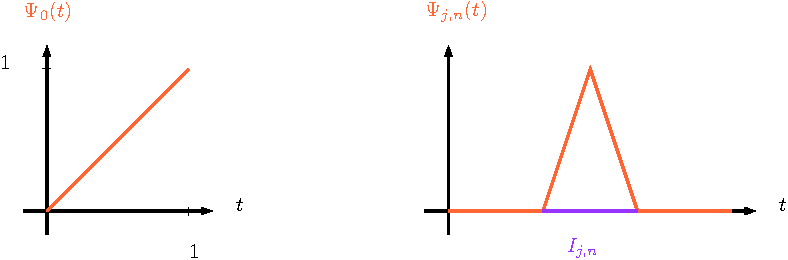
\includegraphics[scale=.9]{figure3.pdf}
\caption{Depiction of $\Psi_0$ and $\Psi_{j,n}$ for the Haar basis.}
\end{figure}
\\
We then realize that $S(t)=\sum_j N_{j,n}\Psi_{j,t}(t)= f_{n+1}(t)-f_n(t)$ as we have defined them in the previous construction. So this construction of $S$ leads exactly to our previous construction of Brownian Motion in the first chapter. 
\newpage
\subsubsection{The Fourier series of $(B_t)_{t \in [0,1]}$ and the Fourier Basis}
In order to motivate the second example of ONB, namely the Fourier basis, we first start with a few considerations. Let us consider a Brownian motion $(B_t)_{t \in [0,1]}$ defined on the time-interval $[0,1]$. We define the Brownian bridge $\beta_t := B_t-tB_1$ (recall that is also a centered Gaussian process) and we know that $\beta$ is independent of $B_1$). Since $\beta$ is almost surely a continuous function with $\beta_0=\beta_1$, we can almost surely decompose it into a Fourier series (in the sense of $L^2$ functions). More precisely, we have for all $t \in [0,1]$, the sequence of functions
\begin{align*}
S_m(t):= \sum_{n=1}^m b_n \sin( \pi n t ), \text{ where } b_n = \int_0^1 \beta_t \sin( \pi n t ) dt. 
\end{align*}
We then have that this sequence $S_m$ converges in $L^2 ([0,1])$ to the function $t \mapsto \beta_t$ as $m \to \infty$. So, if we set $\tilde{b_0}= B_1$ and $\tilde{b}_n = \pi n b_n / \sqrt{2}$, then we obtain 
\begin{align*}
B_t = \tilde{b_0}t + \lim_{m \to \infty} \sum_{n=1}^m \frac{\tilde{b_n} \sqrt{2}}{ \pi n} \sin ( \pi n t ), \tag{$\clubsuit$}
\end{align*}
where the limit is in the sense of $L^2$ limits of functions. \\
\\
We now use the Fourier basis. The ONB of $L^2([0,1])$ is in this case given by $\varphi_0(t)=1$ and for all $n \geq 1$ we set $\varphi_n(t)= \sqrt{2} \cos( \pi t n)$. Consequently,
\begin{align*}
\Psi_0(t)=t, \ \Psi_n(t) = \frac{\sqrt{2}}{\pi n} \sin( \pi n t) \text{ for all } n \geq 1.
\end{align*}
We then know that $S(t):= " \sum N_n \Psi_n(t)"$ has the law of a Brownian motion on $[0,1]$ and
\begin{align*}
S(t)= \sum_{n=1}^\infty  \frac{N_n\sqrt{2}}{ \pi n} \sin( \pi n t) + N_0t, \tag{$\spadesuit$}
\end{align*}
since the Fourier coefficients are unique, by comparison of $(\clubsuit$) with $(\spadesuit)$ we can identify the Fourier coefficients to be independent centered standard Gaussian random variables. 
\end{document}